\chapter{基于拉格朗日乘数的双变量伽辽金法}
\section{}

\section{}

\section{数值算例}
\subsection{一维弹性杆撞击刚性墙实验}

考虑一维弹性杆撞击刚性壁的情况，如图\ref{fg:impact_bar}所示，
弹性杆的材料系数为$E=1$，$\rho=1$，杆长$L=1$。
弹性杆初始具有均匀速度$v_0=1$，撞击时在杆的左端施加位移条件，
要求该端位移在任意时刻都为零，即$(u(x=0,t)=0$)，
杆的右端为自由端。
应力的解析解是一个压缩波，其表达式为$\sigma = EAu_{,x}$。
如图\ref{fg:impact_bar}所示，在弹性杆的左端施加强制边界条件，
而右端则施加自然边界条件。弹性杆的求解域通过图\ref{fg:node model}所示采用
同样密度$(20 × 20)$的三节点和六节点三角形单元网格离散，
但区别在于采用的网格是否均布分别进行离散。

\begin{figure}[!h]
    \centering
    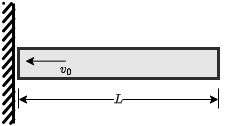
\includegraphics[scale=0.7]{fig/1.png}
\caption{\centering{一维弹性杆撞击刚性墙示意图}}
\label{fg:impact_bar}
\end{figure}

\begin{figure}[!h]
    \centering
        \begin{tabular}{cccc@{\hspace{5pt}}c}
            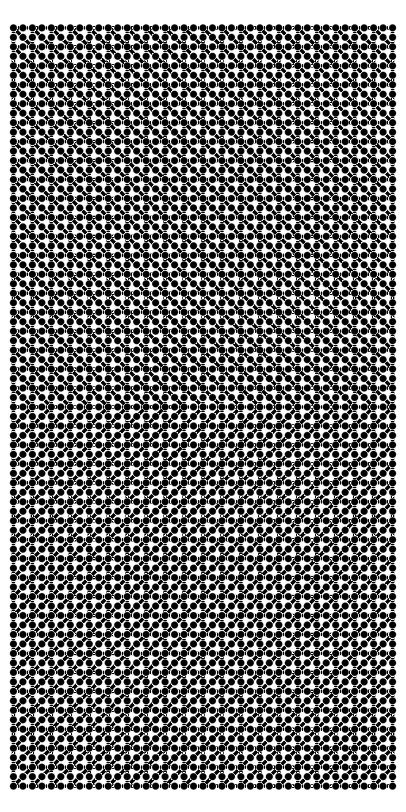
\includegraphics[width=0.21\textwidth]{fig/Tri6_b=2_20.png} &
            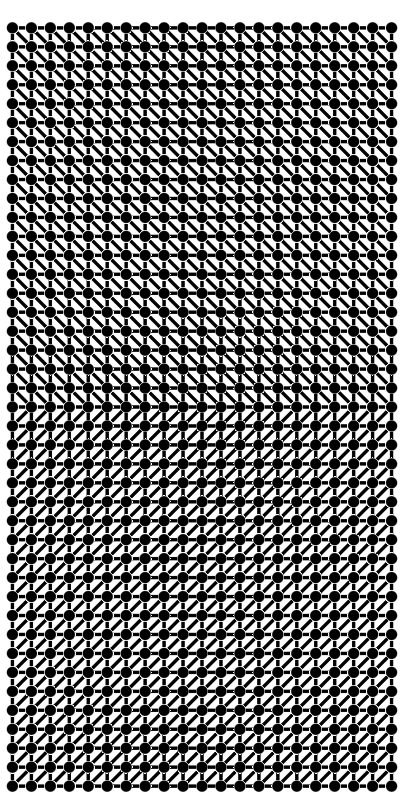
\includegraphics[width=0.21\textwidth]{fig/Tri3_b=2_20.png} &
            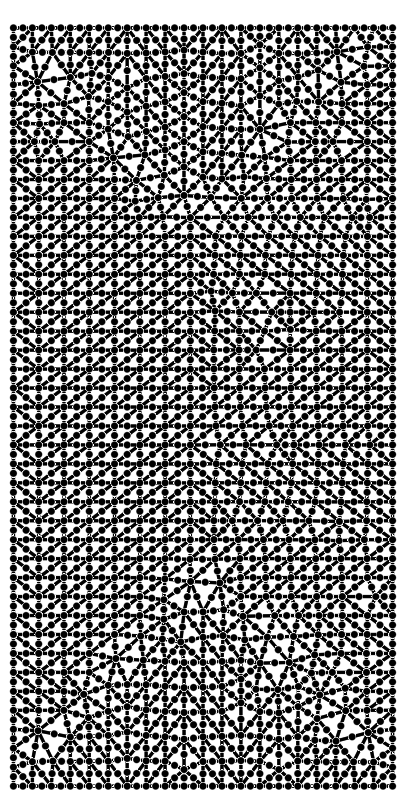
\includegraphics[width=0.21\textwidth]{fig/Tri6非均布_b=2_20.png} &
            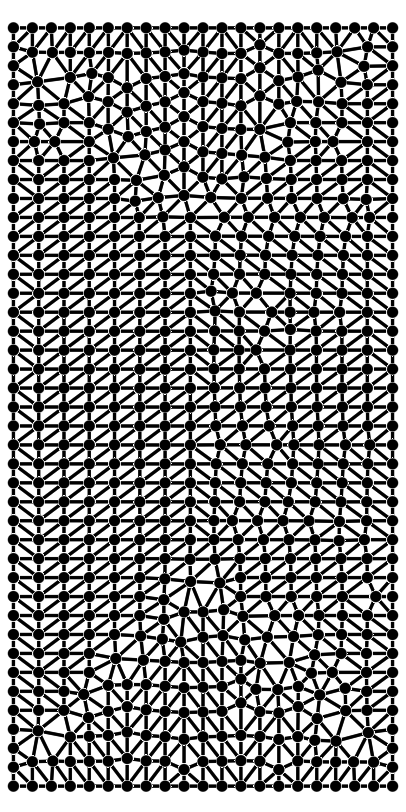
\includegraphics[width=0.21\textwidth]{fig/Tri3非均布_b=2_20.png} \\
            
\includegraphics[width=0.2\textwidth]{fig/Tri6应力图.png} &
            
\includegraphics[width=0.2\textwidth]{fig/Tri3应力图.png} &
            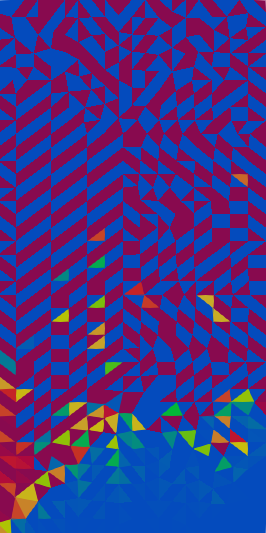
\includegraphics[width=0.2\textwidth]{fig/Tri6应力图非均布.png} &
            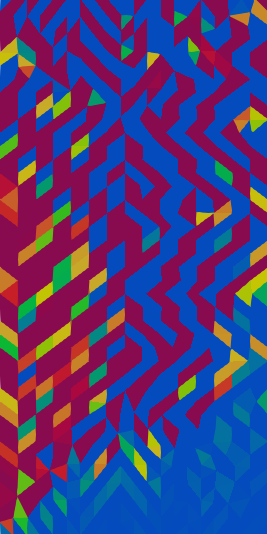
\includegraphics[width=0.2\textwidth]{fig/Tri3应力图非均布.png} &
            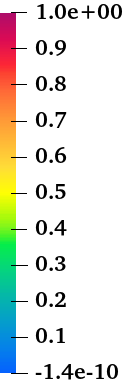
\includegraphics[width=0.1\textwidth]{fig/legend.png} \\
            Tri6均布网格 & Tri3均布网格 & Tri6非均布网格 &  Tri3非均布网格 \\
        \end{tabular}
        \caption{弹性杆问题节点模型以及对应的应力云图}
        \label{fg:node model}
\end{figure}
 
图\ref{fg:node model}为一维弹性杆撞击刚性墙问题的在时空域上的相对应的应力云图。
从图中可以看出采用基于
拉格朗日变分方案的数值分析方法在时空域上求解弹性杆动力学问题时，
求解域只需按照图\ref{fg:node model}所示的均布网格进行离散，
就可以得到稳定的数值求解空间，并且随着时间的增长也不会产生振荡，从而有效的提高了计算精度。




\subsection{一维弹性材料层中的波动问题}
考虑一个厚度为$H=4$的弹性材料层，如图\ref{fg:tension_bar}所示，材料密度$\rho = 1$,弹性模量$E = 1$，波速$\alpha = 1$。
在材料的右侧边界施加位移等于零的强制边界条件。
当$t = 0$时，在材料左边界施加一个持续时间为$1$的压缩应力脉冲$T$，
压缩应力脉冲$T$的示意图为图\ref{fg:impulse wave},表达式为：
\begin{equation}
    T_{11}(0,t)=\begin{cases}
    -\sin(\pi t),& 0\leq t\leq 1,\\
    0,              & 1 < t.
    \end{cases}
\end{equation}

\begin{figure}[!h]
    \centering
    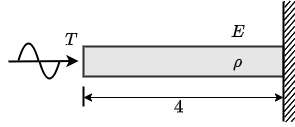
\includegraphics[scale=0.7]{fig/2.png}
\caption{\centering{一维弹性材料层中的波动问题示意图}}
\label{fg:tension_bar}
\end{figure}

\begin{figure}[!h]
    \centering
    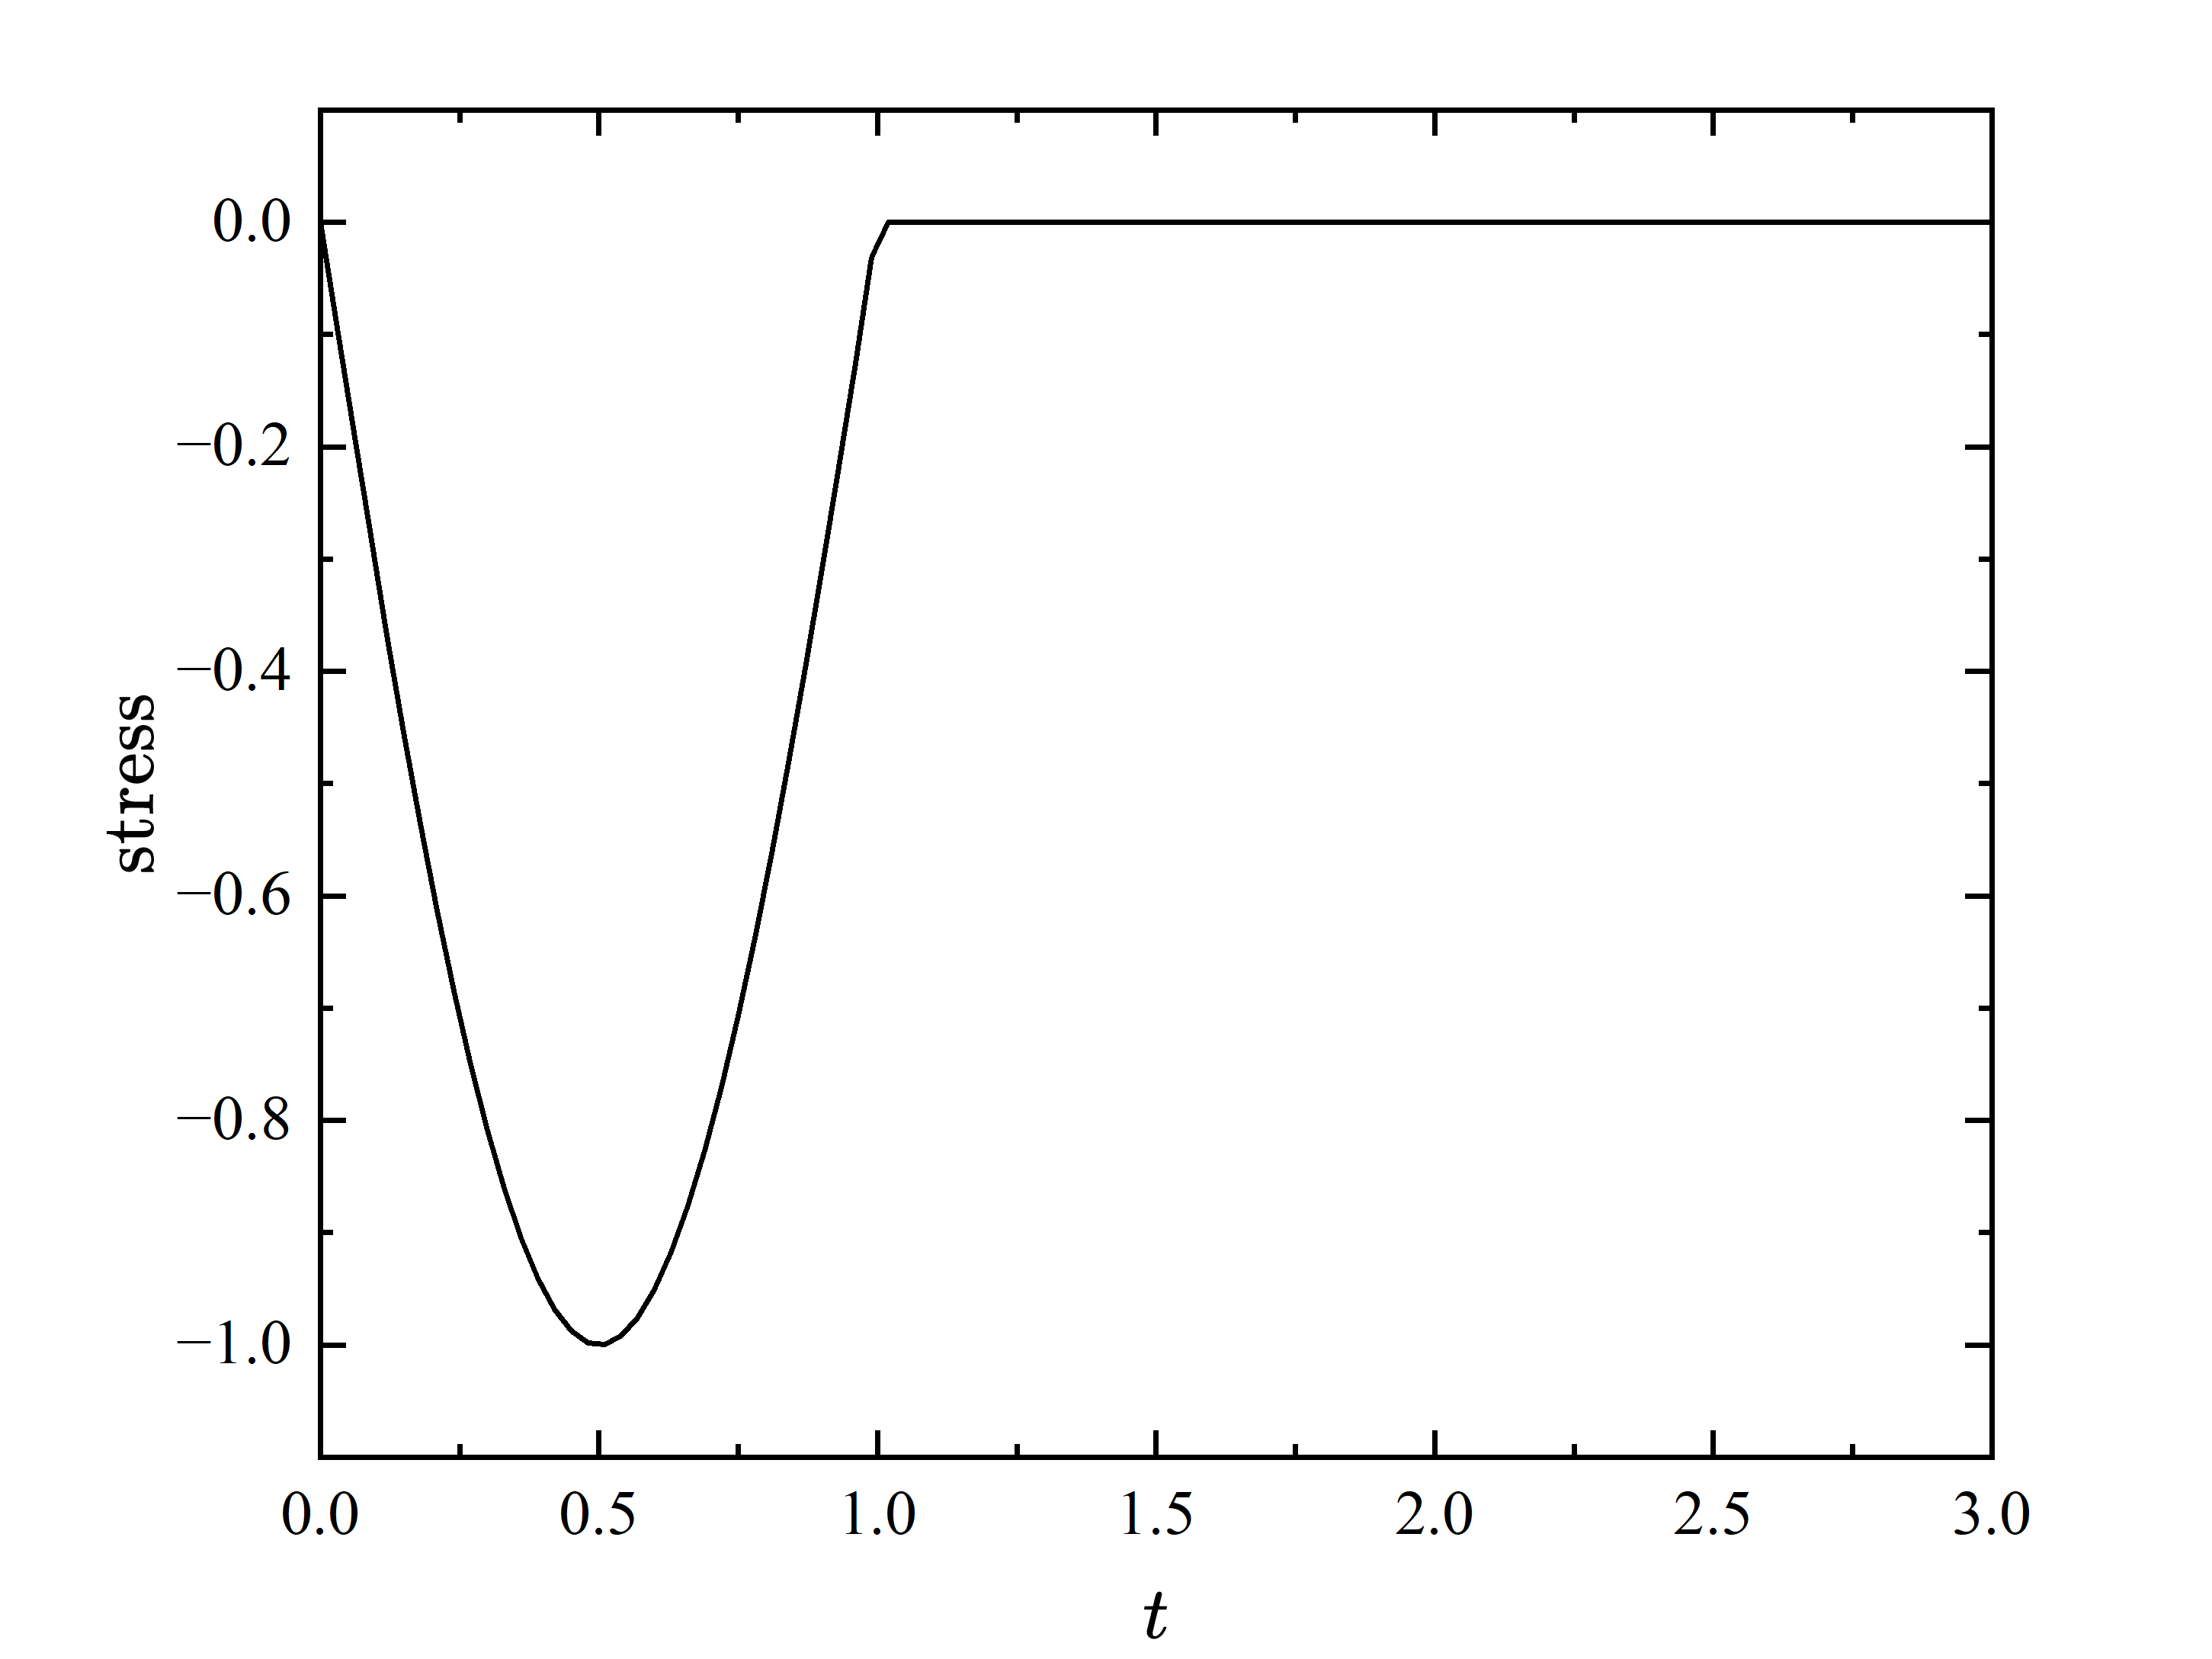
\includegraphics[scale=0.4]{fig/脉冲图.png}
\caption{\centering{施加在弹性材料左侧的应力}}
\label{fg:impulse wave}
\end{figure}

在此脉冲边界条件的影响下，位移的精确解的解析表达式为：
\begin{equation}
  u_1(x_1,t)=
    \begin{cases}
      \frac{2\alpha}{\pi}, & x_1 < \alpha(t - 1),\\
      \frac{\alpha}{\pi}\left[1 - \cos\left(\pi\left(t - \frac{x_1}{\alpha}\right)\right)\right], & \alpha(t - 1) \leq x_1 \leq \alpha t,\\
       0, & \alpha t < x_1.
    \end{cases}
\end{equation}

\begin{figure}[!h]
    \centering
        \begin{tabular}{c@{\hspace{20pt}}c}
            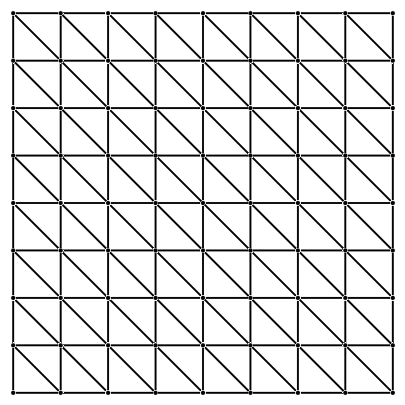
\includegraphics[width=0.3\textwidth]{fig/Tri3_square_8.png} &
            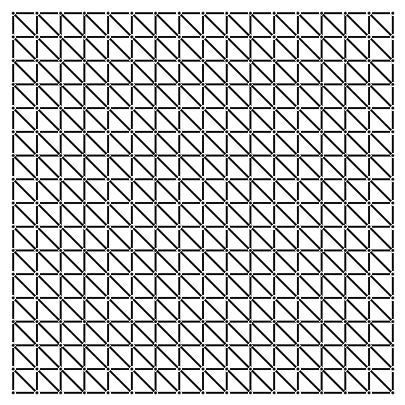
\includegraphics[width=0.3\textwidth]{fig/Tri3_square_16.png} \\
            $9\times9$ & $17\times17$ \\
            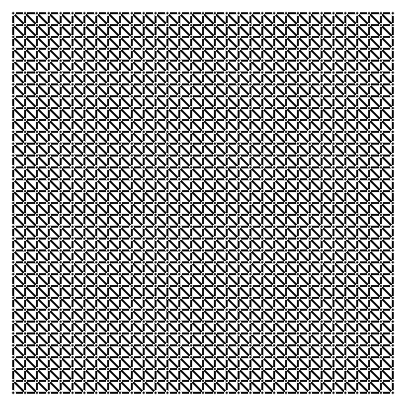
\includegraphics[width=0.3\textwidth]{fig/Tri3_square_32.png} &
            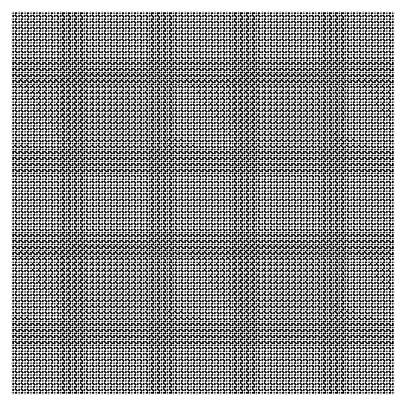
\includegraphics[width=0.3\textwidth]{fig/Tri3_square_64.png} \\
            $33\times33$ & $65\times65$ \\
        \end{tabular}
        \caption{弹性材料波动问题节点模型}\label{fg:square node model}
\end{figure}

弹性材料的求解域分别通过图\ref{fg:square node model}所示采用均布的四个疏密不同、
三节点三角形单元网格进行离散。
图\ref{fg:ecr}为采用上述四个疏密不同的离散节点时的位移误差和能量误差的收敛结果。
从图中可以看出采用基于
拉格朗日变分方案的数值分析方法在时空域上求解弹性材料波动问题时， 
其位移误差和能量误差均能达到理论收敛率。
\begin{figure}[!h]
    \centering
    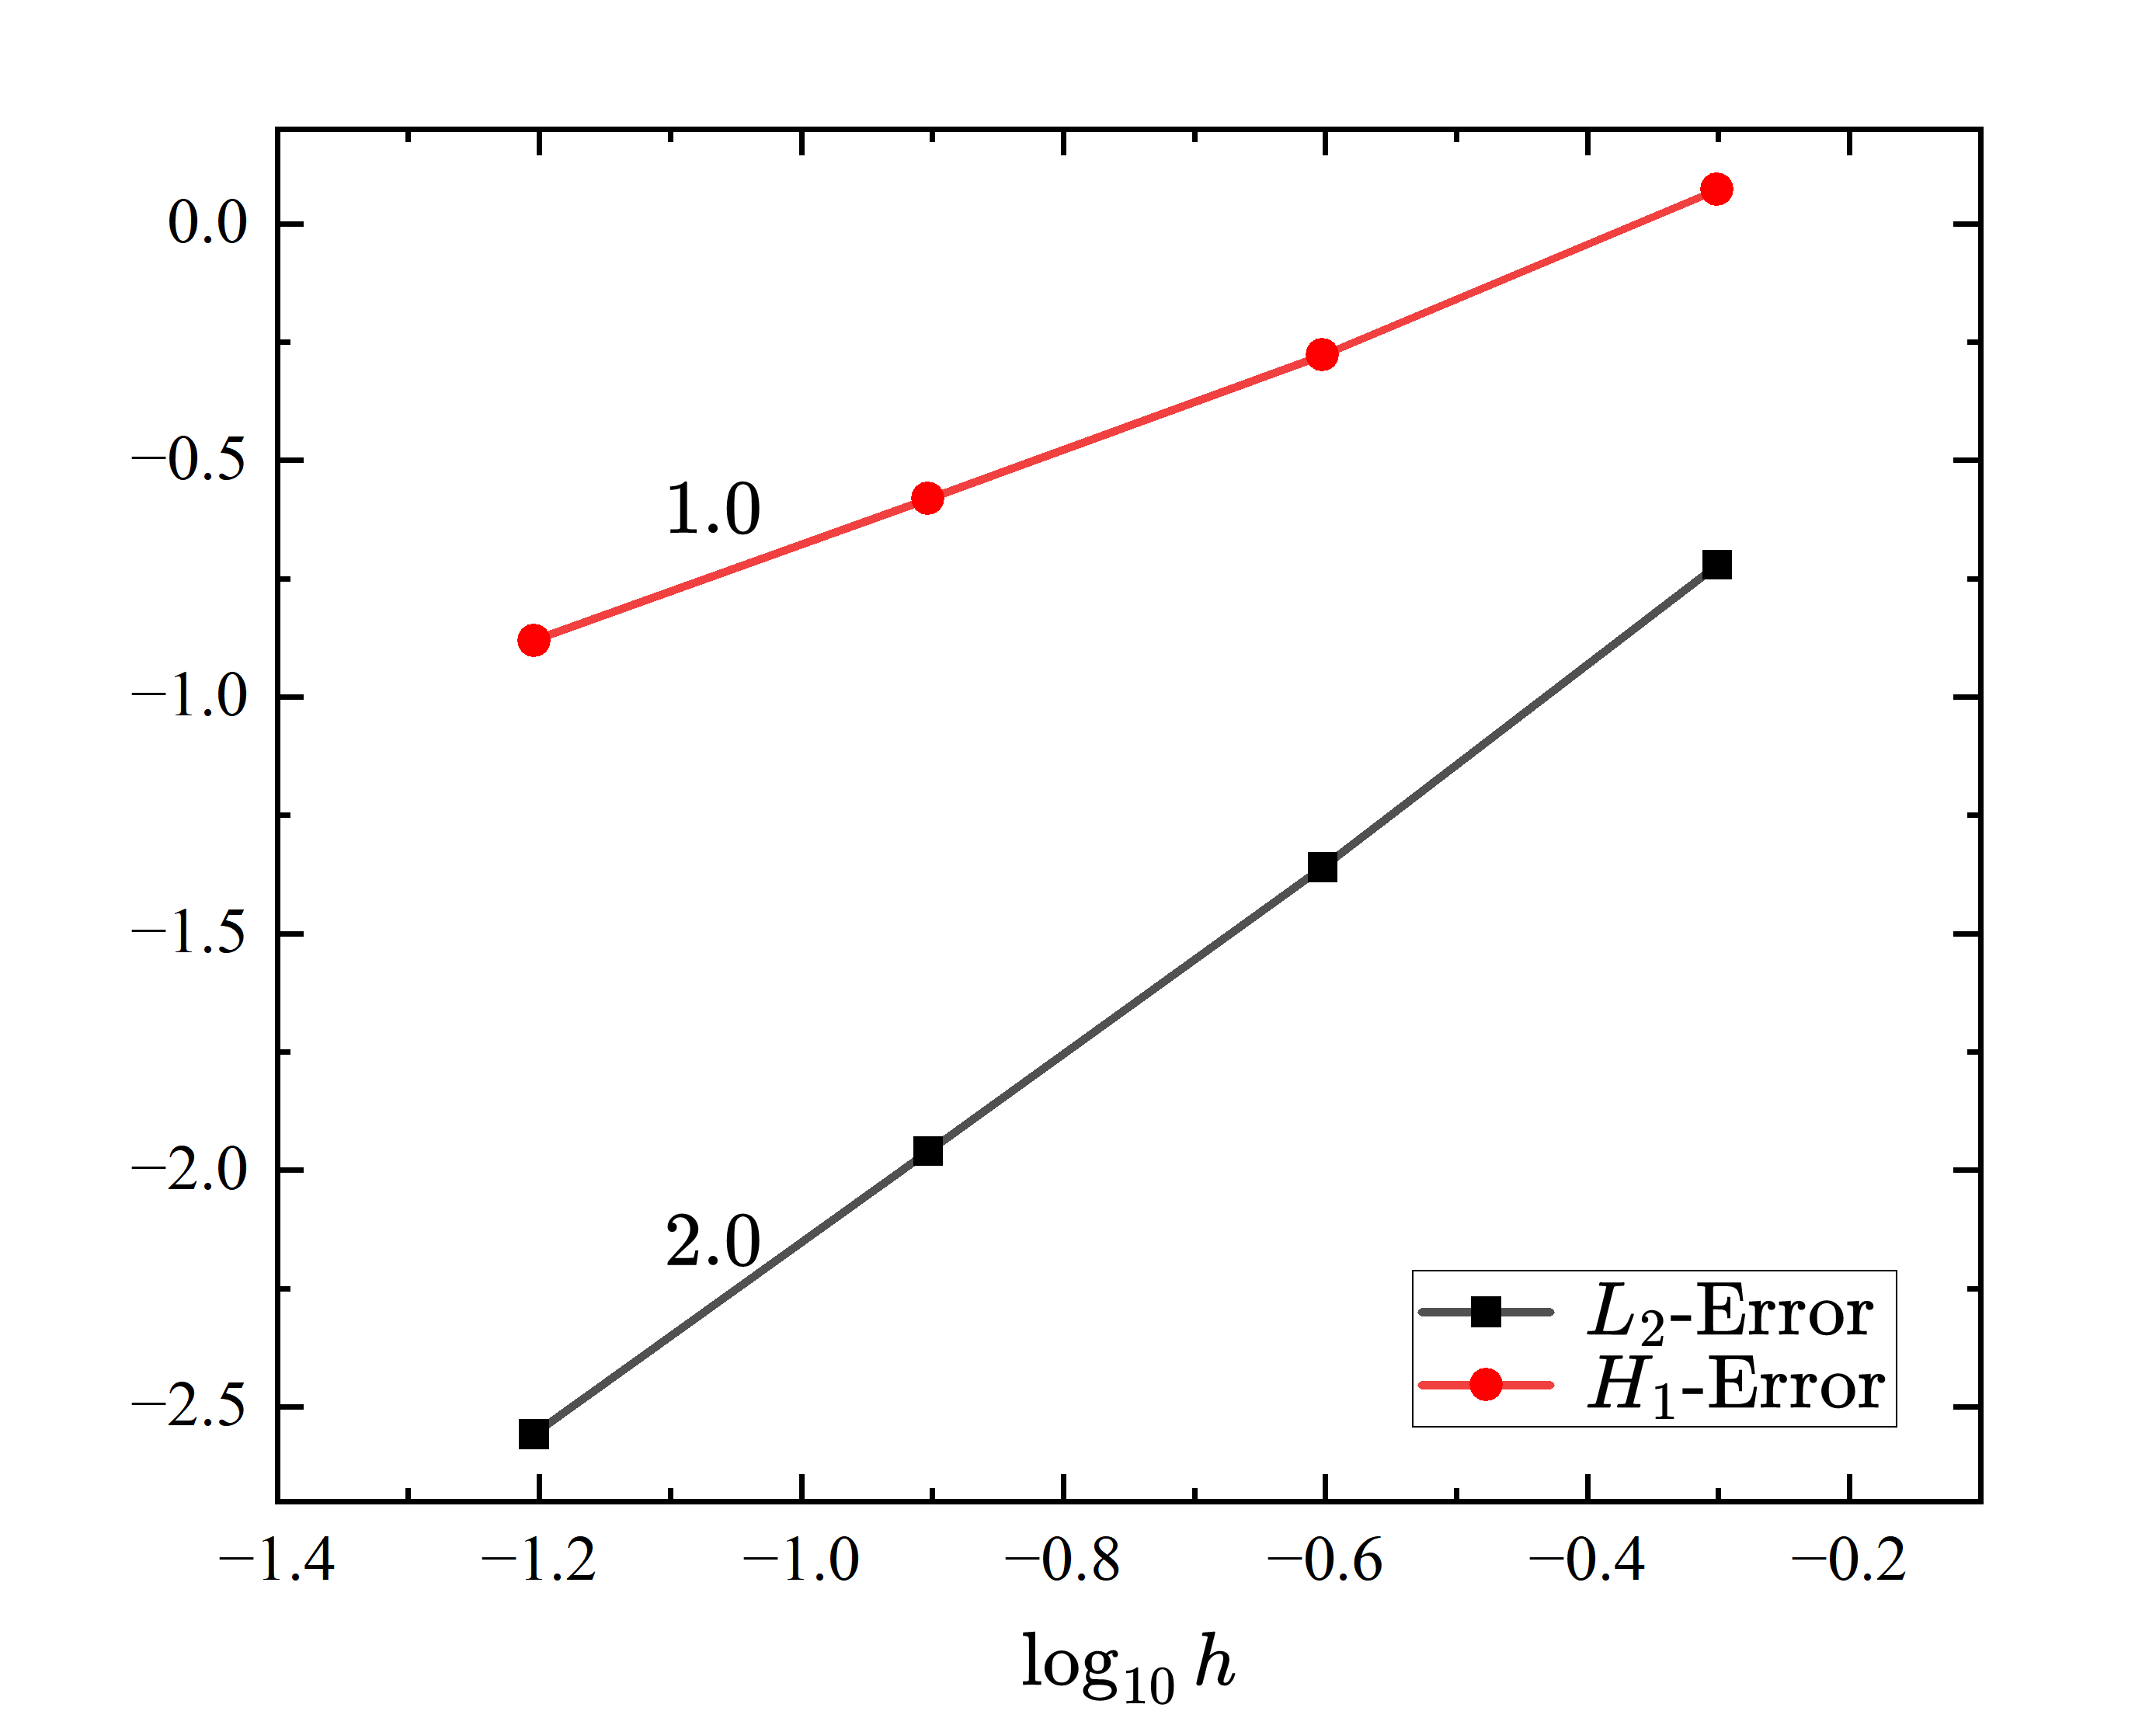
\includegraphics[scale=0.38]{fig/Tri3均布误差收敛率.png}
\caption{\centering{一维弹性材料波动问题采用Tri3单元计算的误差收敛结果}}
\label{fg:ecr}
\end{figure}

当采用自由度更高的三角形Hermite单元拉进行计算和上面相同的均布网格，
能得到精度更高的误差收敛率，如图\ref{fg:Hecr}所示：
位移误差收敛率达到了2.7，能量误差收敛率达到了1.6。

\begin{figure}[!h]
    \centering
    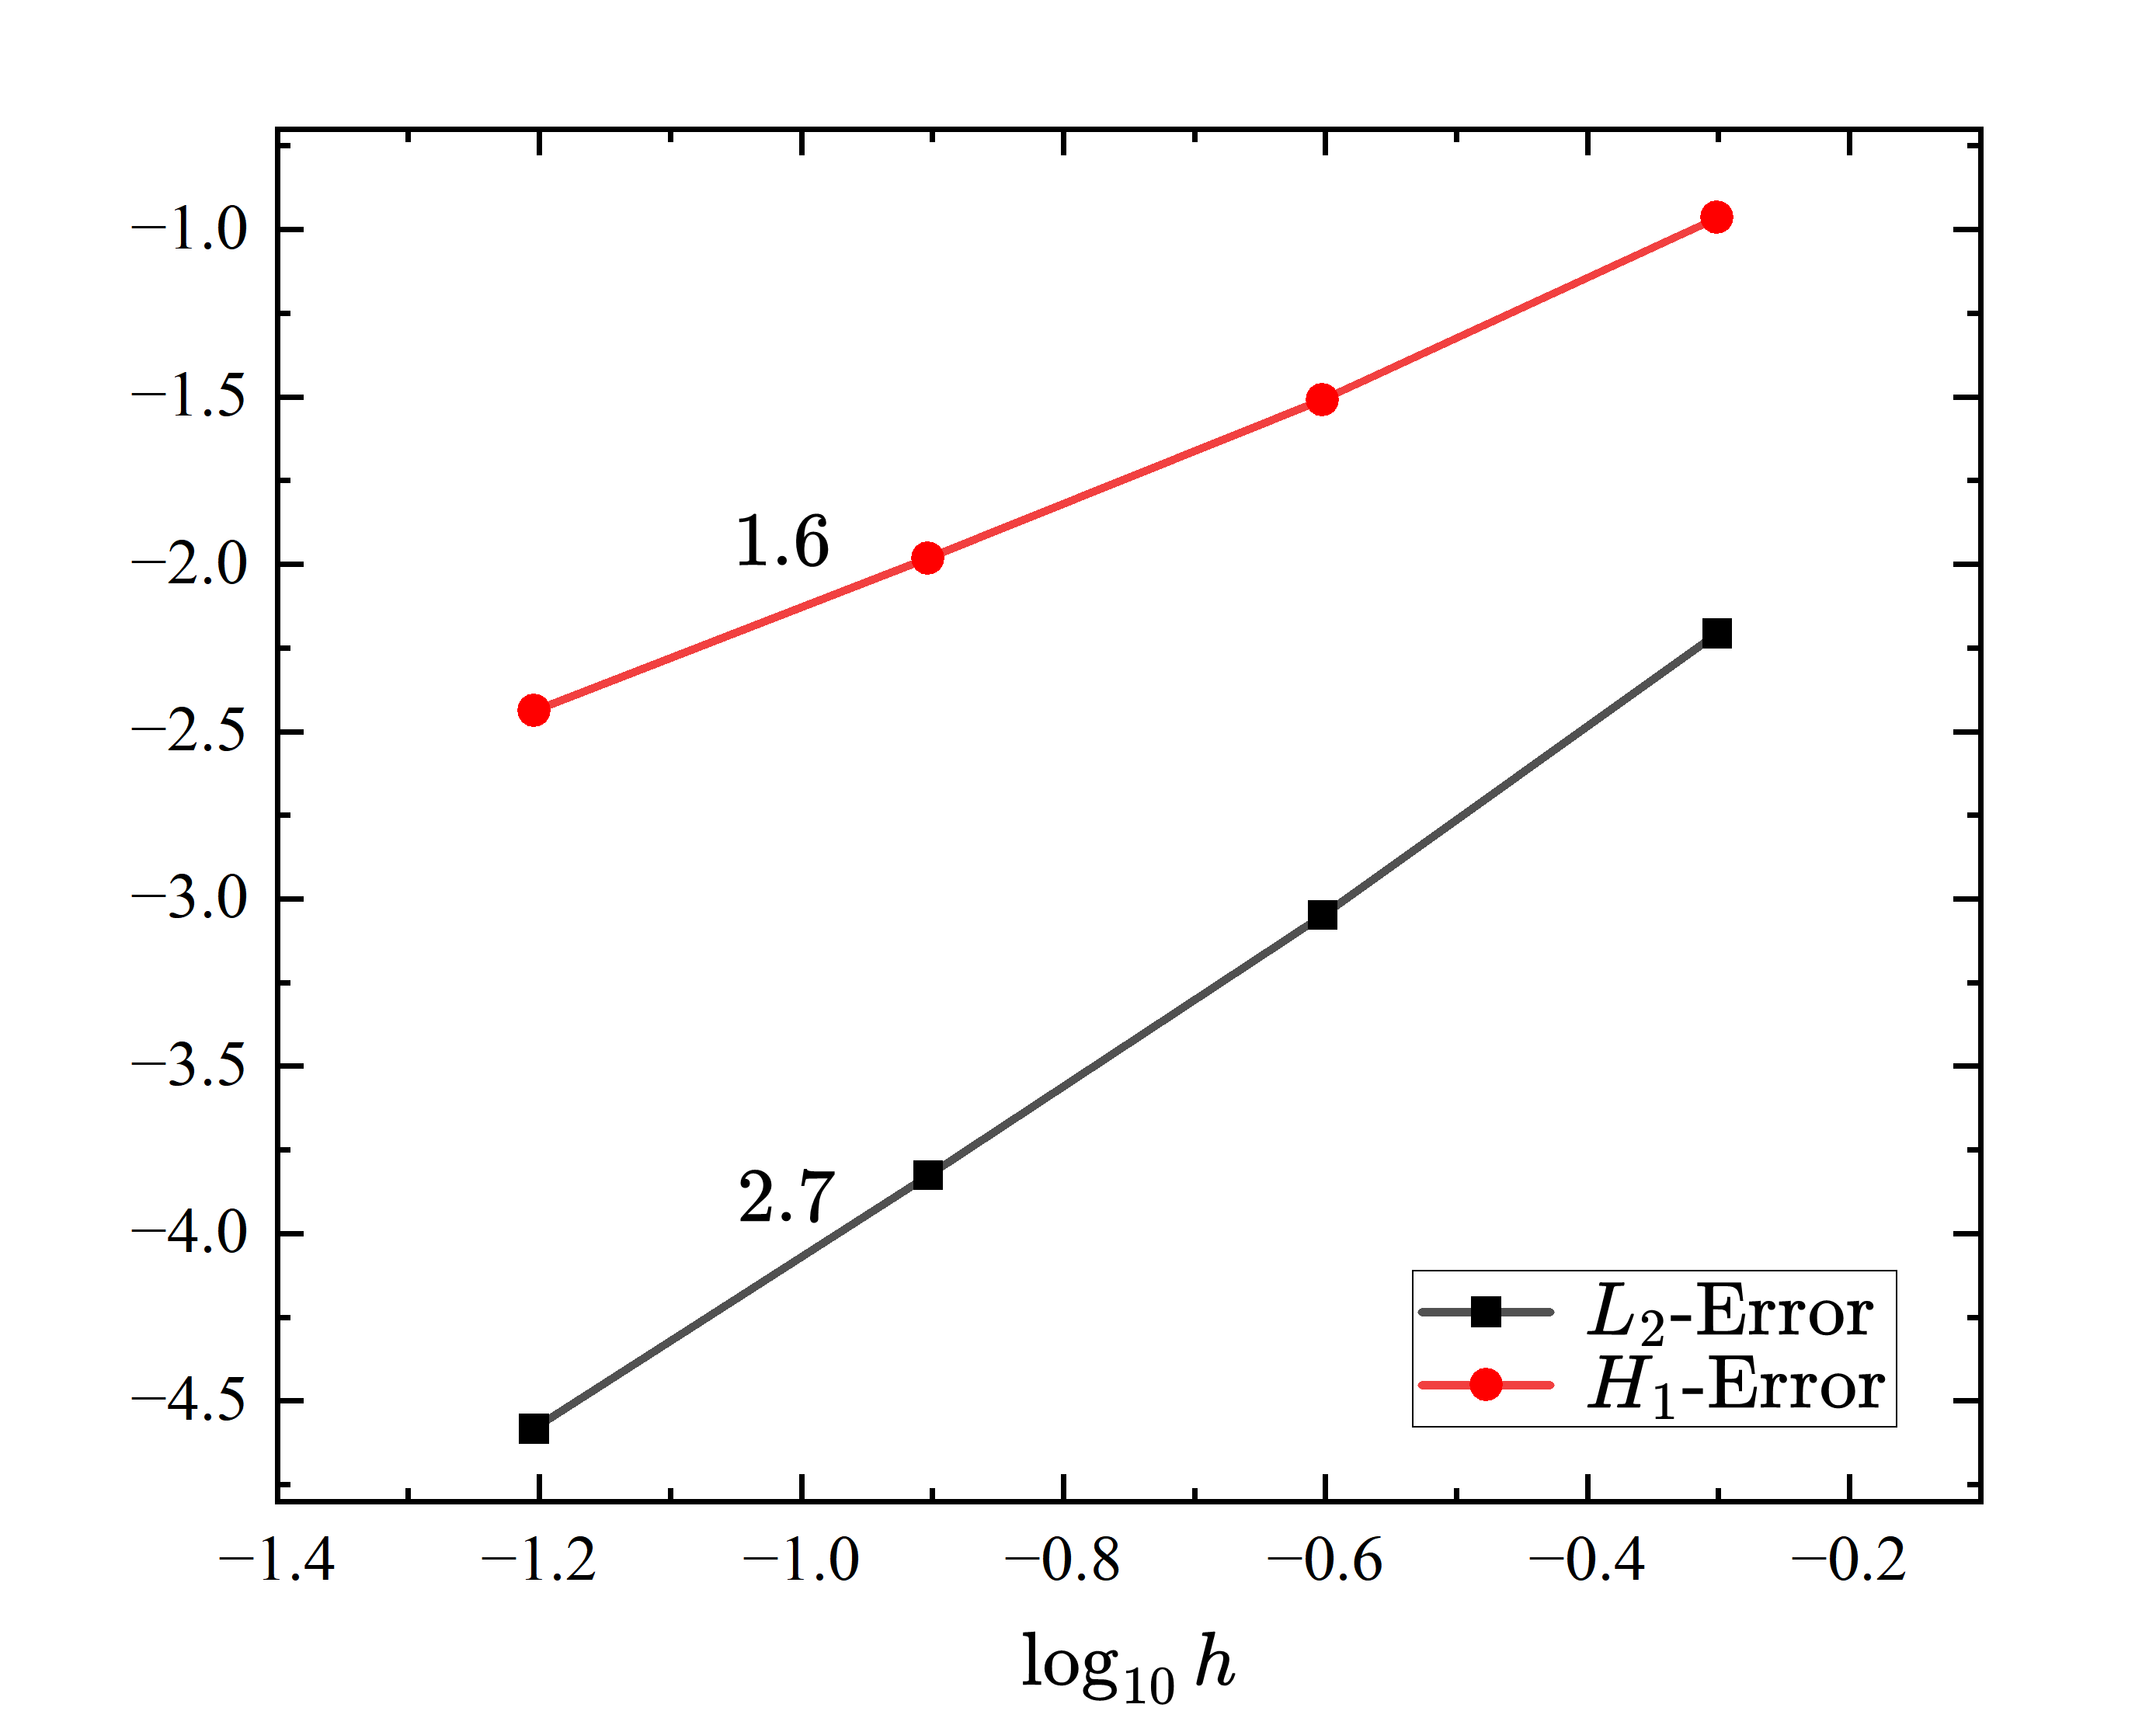
\includegraphics[scale=0.38]{fig/Hermite均布误差收敛率.png}
\caption{\centering{一维弹性材料波动问题采用Hermite单元计算的误差收敛结果}}
\label{fg:Hecr}
\end{figure}

图\ref{fg:3dd}为采用离散密度相同($20\times20$)的三角形单元，但离散方式不同，
分为均布网格和非均布网格两种形式进行离散得到的三维位移图。
\begin{figure}[!h]
    \centering
        \begin{tabular}{c@{\hspace{20pt}}c}
            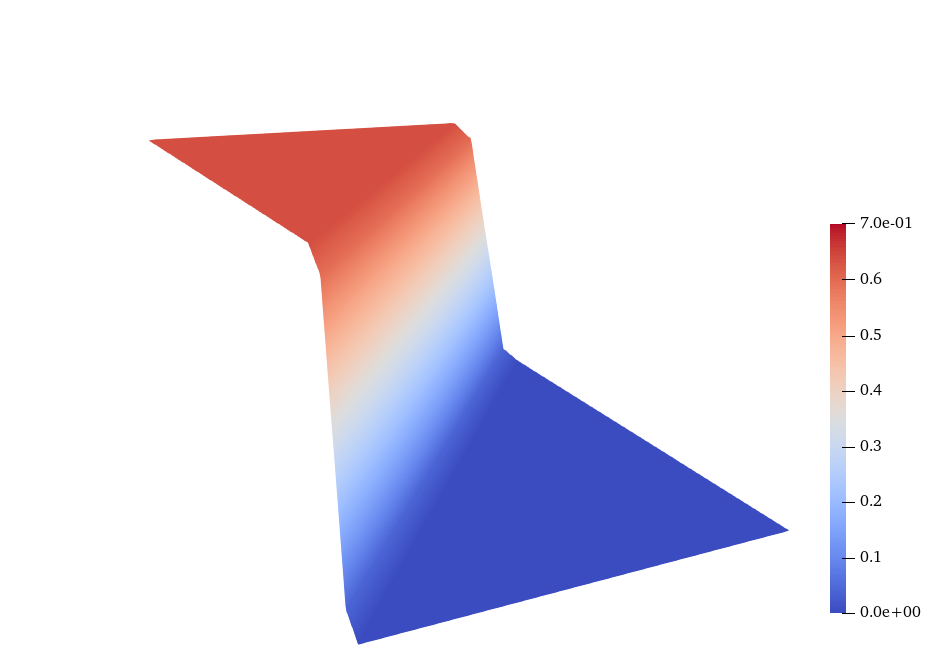
\includegraphics[width=0.5\textwidth]{fig/Tri3三维位移图20.png} &
            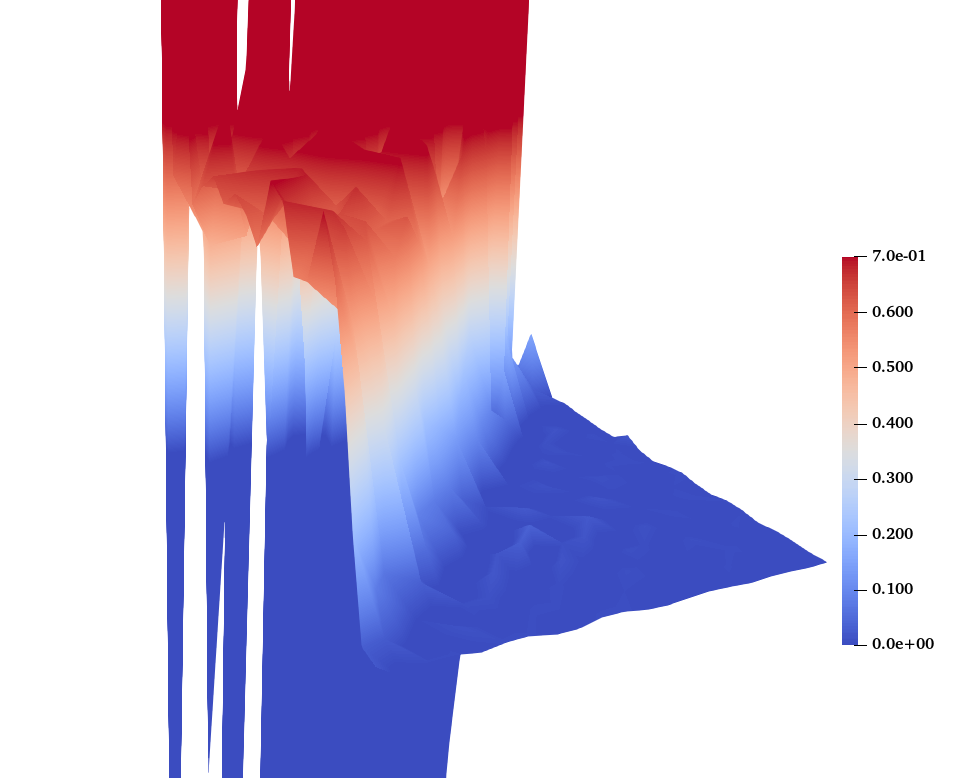
\includegraphics[width=0.5\textwidth]{fig/Tri3非均布三维位移图20.png} \\
            $均布网格$ & $非均布网格$ \\
        \end{tabular}
        \caption{弹性材料波动问题三维位移图}\label{fg:3dd}
\end{figure}

一维弹性材料波动问题在非均布的网格节点上进行计算时会产生较大的振荡现象，
为解决这一问题，尝试换用自由度更高的Hermite单元进行计算，
并对非均布网格适当的局部加密。
如图\ref{fg:local}所示，对20*20的非均布网格在解的坡顶进行局部加密，
来缓解梯度变化带来的振荡现象，从而得到更加稳定的数值解。
\begin{figure}[!h]
    \centering
        \begin{tabular}{c@{\hspace{20pt}}c}
            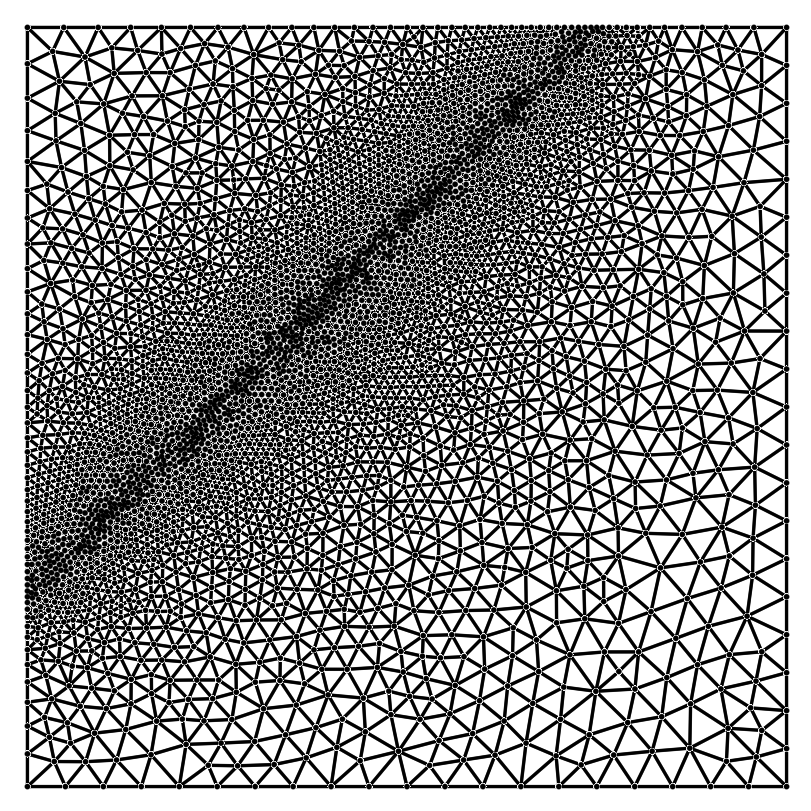
\includegraphics[width=0.4\textwidth]{fig/Tri3非均布_Jbjm_0.03.png} &
            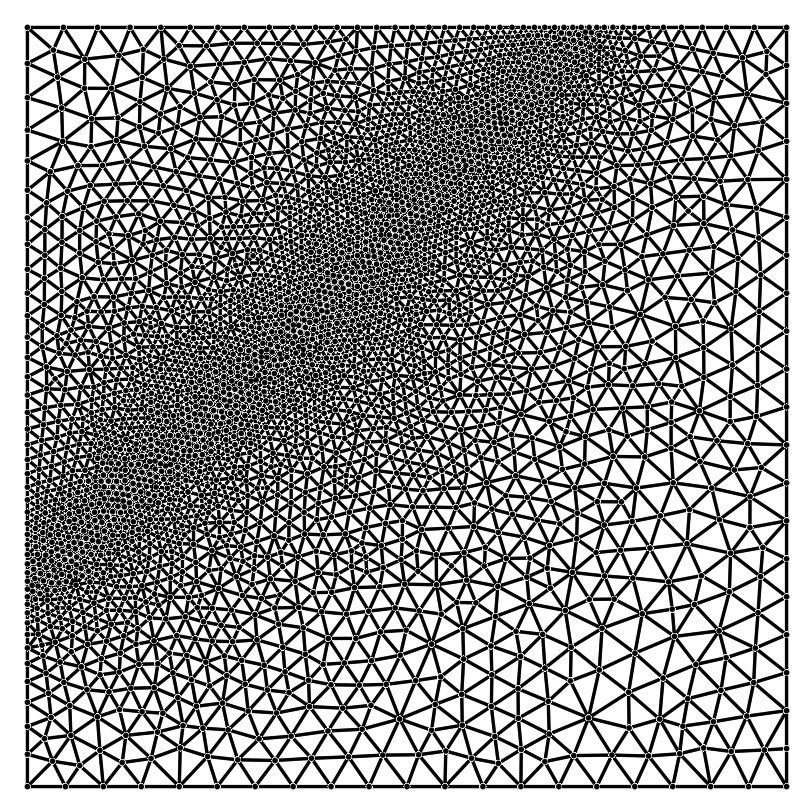
\includegraphics[width=0.4\textwidth]{fig/Tri3非均布_Jbjm_0.04.png} \\
            $c=0.03$网格示意图 & $c=0.04$网格示意图  \\
            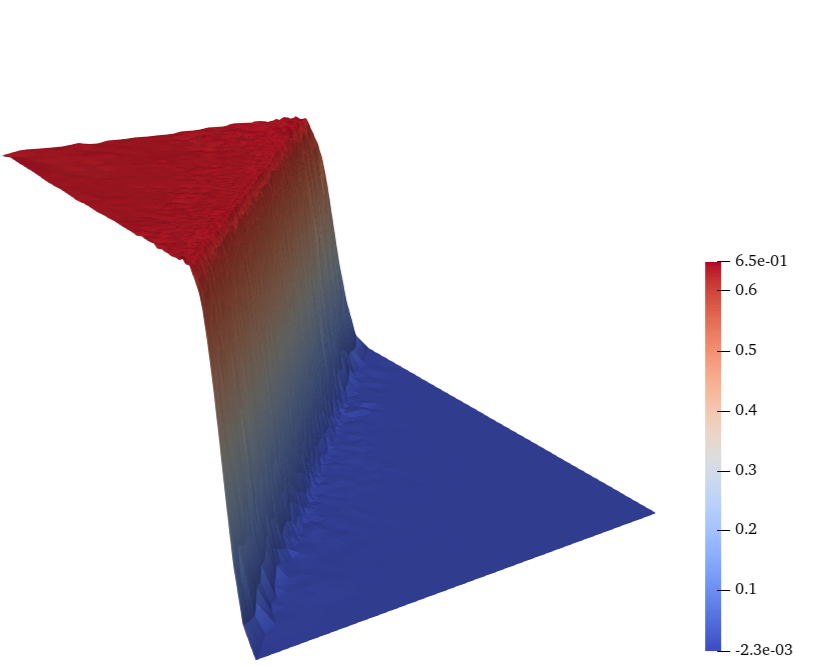
\includegraphics[width=0.5\textwidth]{fig/C=0.2_c=0.03.png} &
            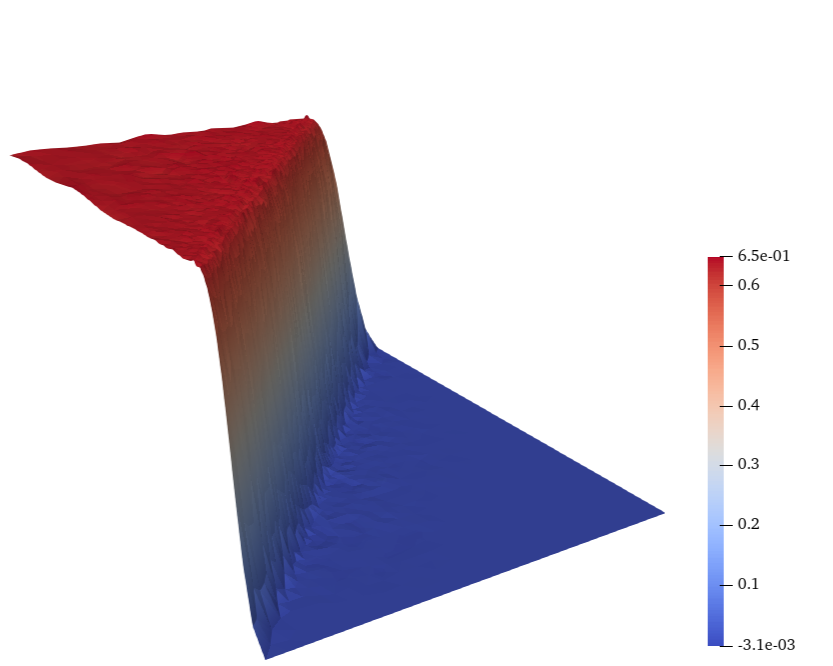
\includegraphics[width=0.5\textwidth]{fig/C=0.2_c=0.04.png} \\
            $c=0.03$位移图 & $c=0.04$位移图 \\
        \end{tabular}
        \caption{弹性材料波动问题局部加密采用Hermite单元计算的三维位移图}\label{fg:local}
\end{figure}
